%!TEX encoding = UTF-8 Unicode
% -*- coding: UTF-8; -*-
% vim: set fenc-utf-8

\chapter{Maquette des interfaces}
\label{s:maquettes_interfaces}

Ce chapitre présente les maquettes des principales interfaces de l'application VisuaLigue.
Une courte explication des fonctionnalités moins évidentes est également présente à la suite des figures si nécessaire.

\begin{figure}[htpb]
    \centering
    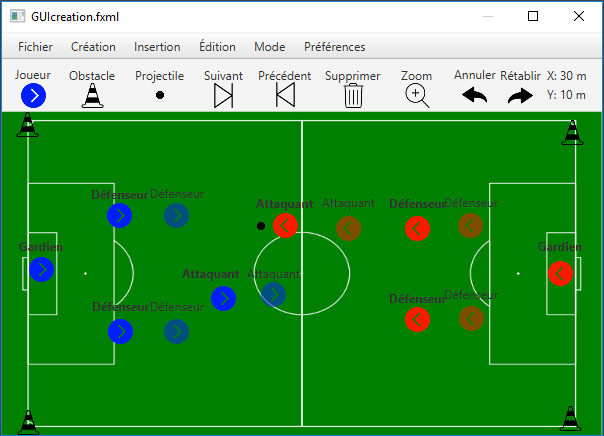
\includegraphics[scale=0.7]{fig/gui/gui_creation.png}
    \caption{Interface pour la création des stratégies}
    \label{fig:gui:gui_creation}
\end{figure}

Cette interface permet l'édition des stratégies, soit en mode image par image ou en mode temps réel.
Les trois premiers icônes en partant de la gauche permettent de glisser des éléments sur le terrain.
Les icônes "suivant" et "précédent" permettent respectivement d'avancer ou de reculer d'une image dans le mode image par image.
Les étiquettes "x" et "y" à la droite des icônes correspondent aux coordonnées de la souris sur le terrain en unités réelles.
La transparence de certains joueurs sur la figure ci-dessus correspond à des éléments qui proviennent d'une image précédente lors de l'édition en mode image par image.

\begin{figure}[htpb]
    \centering
    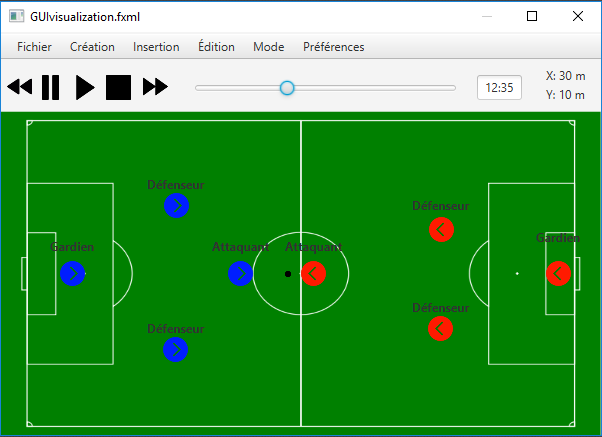
\includegraphics[scale=0.7]{fig/gui/gui_visualisation.png}
    \caption{Interface pour la visualisation des stratégies}
    \label{fig:gui:gui_visualisation}
\end{figure}

Cette interface permet la visualisation des stratégies préalablement créées. 
En plus des boutons habituels de visionnement de vidéos, on y retrouve un curseur glissant permettant de se déplacer facilement à n'importe quel temps de la stratégie.
Ce temps peut aussi être modifié directement dans la boîte de saisie prévue à cet effet à la droite du curseur.
Les coordonnées de la souris sont encore affichées.

\begin{figure}[htpb]
    \centering
    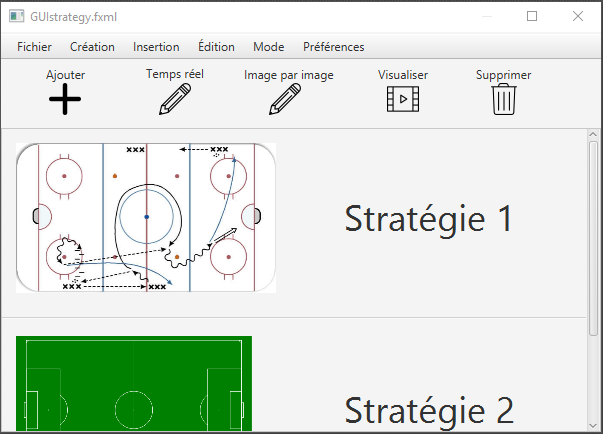
\includegraphics[scale=0.7]{fig/gui/gui_strategie.png}
    \caption{Interface de gestion des stratégies}
    \label{fig:gui:gui_strategie}
\end{figure}

Cette interface permet la gestion des stratégies.
Après avoir sélectionné une stratégie, une multitude de choix s'offre à l'entraineur. 
Il peut supprimer la stratégie, la visionner, ou bien l'éditer soit en mode temps réel ou en mode image par image. 
Bien sûr, l'interface permet aussi l'ajout d'une nouvelle stratégie.

\begin{figure}[htpb]
    \centering
    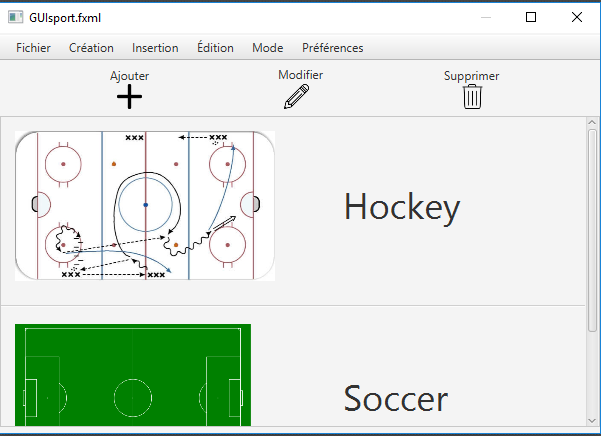
\includegraphics[scale=0.7]{fig/gui/gui_sport.png}
    \caption{Interface de gestion des sports}
    \label{fig:gui:gui_sport}
\end{figure}

Cette interface permet la gestion des sports.
Il est possible d'ajouter, de modifier ou de supprimer un sport.

\begin{figure}[htpb]
    \centering
    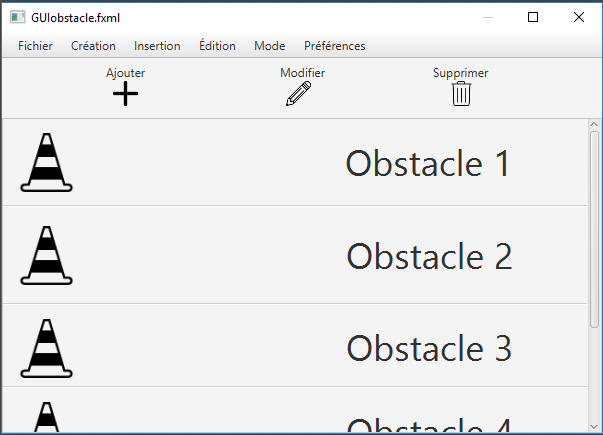
\includegraphics[scale=0.7]{fig/gui/gui_obstacles.png}
    \caption{Interface de gestion des obstacles}
    \label{fig:gui:gui_obstacles}
\end{figure}

Cette interface permet la gestion des obstacles.
Les fonctionnalités sont les mêmes que pour la gestion des stratégies.

\begin{figure}[htpb]
    \centering
    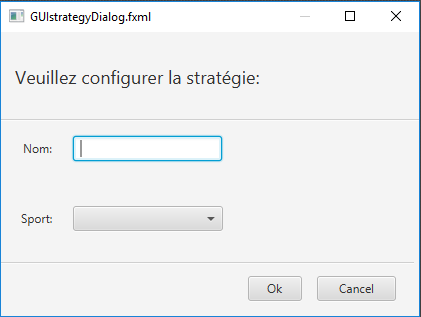
\includegraphics[scale=0.7]{fig/gui/gui_strategie_dialog.png}
    \caption{Interface de configuration des stratégies}
    \label{fig:gui:gui_strategie_dialog}
\end{figure}

Cette fenêtre de dialogue permet de configurer une stratégie.
Elle apparaît lorsque l'on modifie ou ajoute une stratégie via la fenêtre de gestion des stratégies.
On y retrouve une boîte de saisie pour le nom de la stratégie et une boîte de choix pour y associer un sport préalablement créé.

\begin{figure}[htpb]
    \centering
    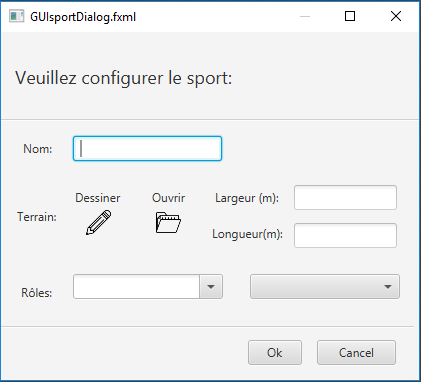
\includegraphics[scale=0.7]{fig/gui/gui_sport_dialog.png}
    \caption{Interface de configuration des sports}
    \label{fig:gui:gui_sport_dialog}
\end{figure}

Cette fenêtre de dialogue permet de configurer un sport.
Elle apparaît lorsque l'on modifie ou ajoute un sport via la fenêtre de gestion des sports.
On y retrouve entre autres deux icônes pour dessiner le terrain ou choisir une image déjà existante.
Deux autres champs permettent la saisie des dimensions réelles du terrain.
Finalement, on peut créer ou choisir un rôle parmi ceux déjà créés afin d'établir la liste des catégories de joueur pour le sport.

\begin{figure}[htpb]
    \centering
    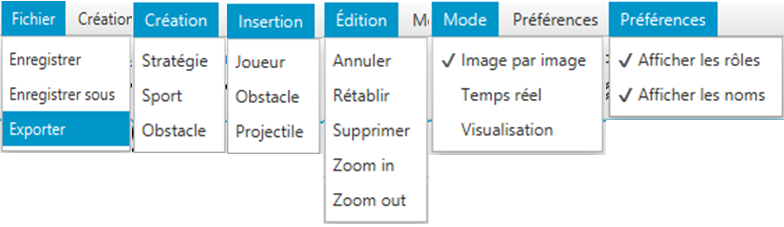
\includegraphics[scale=0.7]{fig/gui/gui_menu.png}
    \caption{Interface du menu pour montrer les options}
    \label{fig:gui:gui_menu}
\end{figure}

Cette figure montre toutes les options du menu présent dans les principales interfaces.
La majorité des fonctionnalités du logiciel sont accessibles par ce menu.
Il est important de comprendre que le sous-menu "mode" ne permet pas le choix de plus d'une option à la fois, contrairement au sous-menu préférences.
